Analise a figura abaixo, e corrija o texto explicativo desta ilustração.
Reescreva o texto \textit{grifando} o que você corrigiu:

\begin{center}
	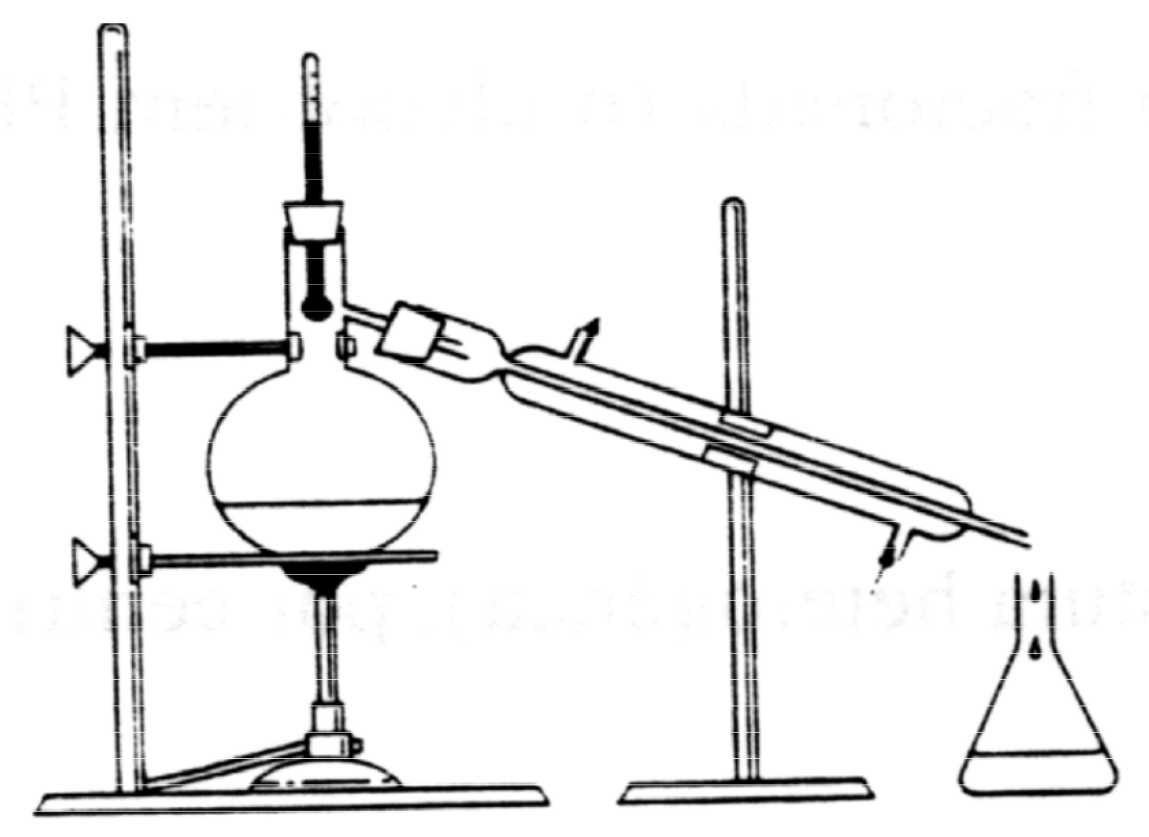
\includegraphics[width = 7cm]{figure.png}
\end{center}

A destilação fracionada é um processo de separação que se baseia na densidade dos componentes de uma mistura sólida.
A solução é aquecida até a ebulição, ocorrendo a vaporização apenas da fase que possui menor densidade.
O vapor, ao ser expulso do balão volumétrico, dirige-se para a coluna de fracionamento, que é refrigerado com água;
a água entra pela parte superior da coluna de fracionamento, resfriando o vapor que retorna ao estado sólido.
Este sólido é recolhido num balão de destilação.
